\documentclass[journal]{IEEEtran}
\usepackage[a5paper, margin=10mm]{geometry}
\usepackage{tfrupee} % Include tfrupee package
\usepackage{gvv-book}
\usepackage{gvv}
\usepackage{pdfpages}
\usepackage{fbox} % For extended fbox features

\setlength{\intextsep}{10pt} % Space between text and floats

\setlength{\headheight}{1cm} % Set the height of the header box
\setlength{\headsep}{0mm}     % Set the distance between the header box and the top of the text

\makeindex
\begin{document}
	
	\bibliographystyle{IEEEtran}
	\onecolumn
	
	\title{
		CALCULATOR
		
		\large{EE1003 : Scientific Programming for Electrical Engineers}
		
		Indian Institute of Technology Hyderabad
	}
	
	\author{Yellanki Siddhanth (EE24BTECH11059)}
	
	\maketitle
	
	\renewcommand{\thefigure}{\theenumi}
	\renewcommand{\thetable}{\theenumi}
	
	\section{Introduction}
	This report describes a calculator system that utilizes a 16x2 LCD display and a pair of 4-button D-pads for user input. The system supports multiple modes for numbers, operators, functions, and inverse functions, providing a versatile and user-friendly interface.
	
	\section{System Components}
	The calculator system consists of the following components:
	\begin{enumerate}
		\item Arduino Atmel328P Microcontroller
		\item 16x2 LCD Display
		\item Two 4-Button D-Pads - 8 Push Buttons
		\item Wires
	\end{enumerate}
		\includepdfset{pages=-} % Include all pages from the PDF
	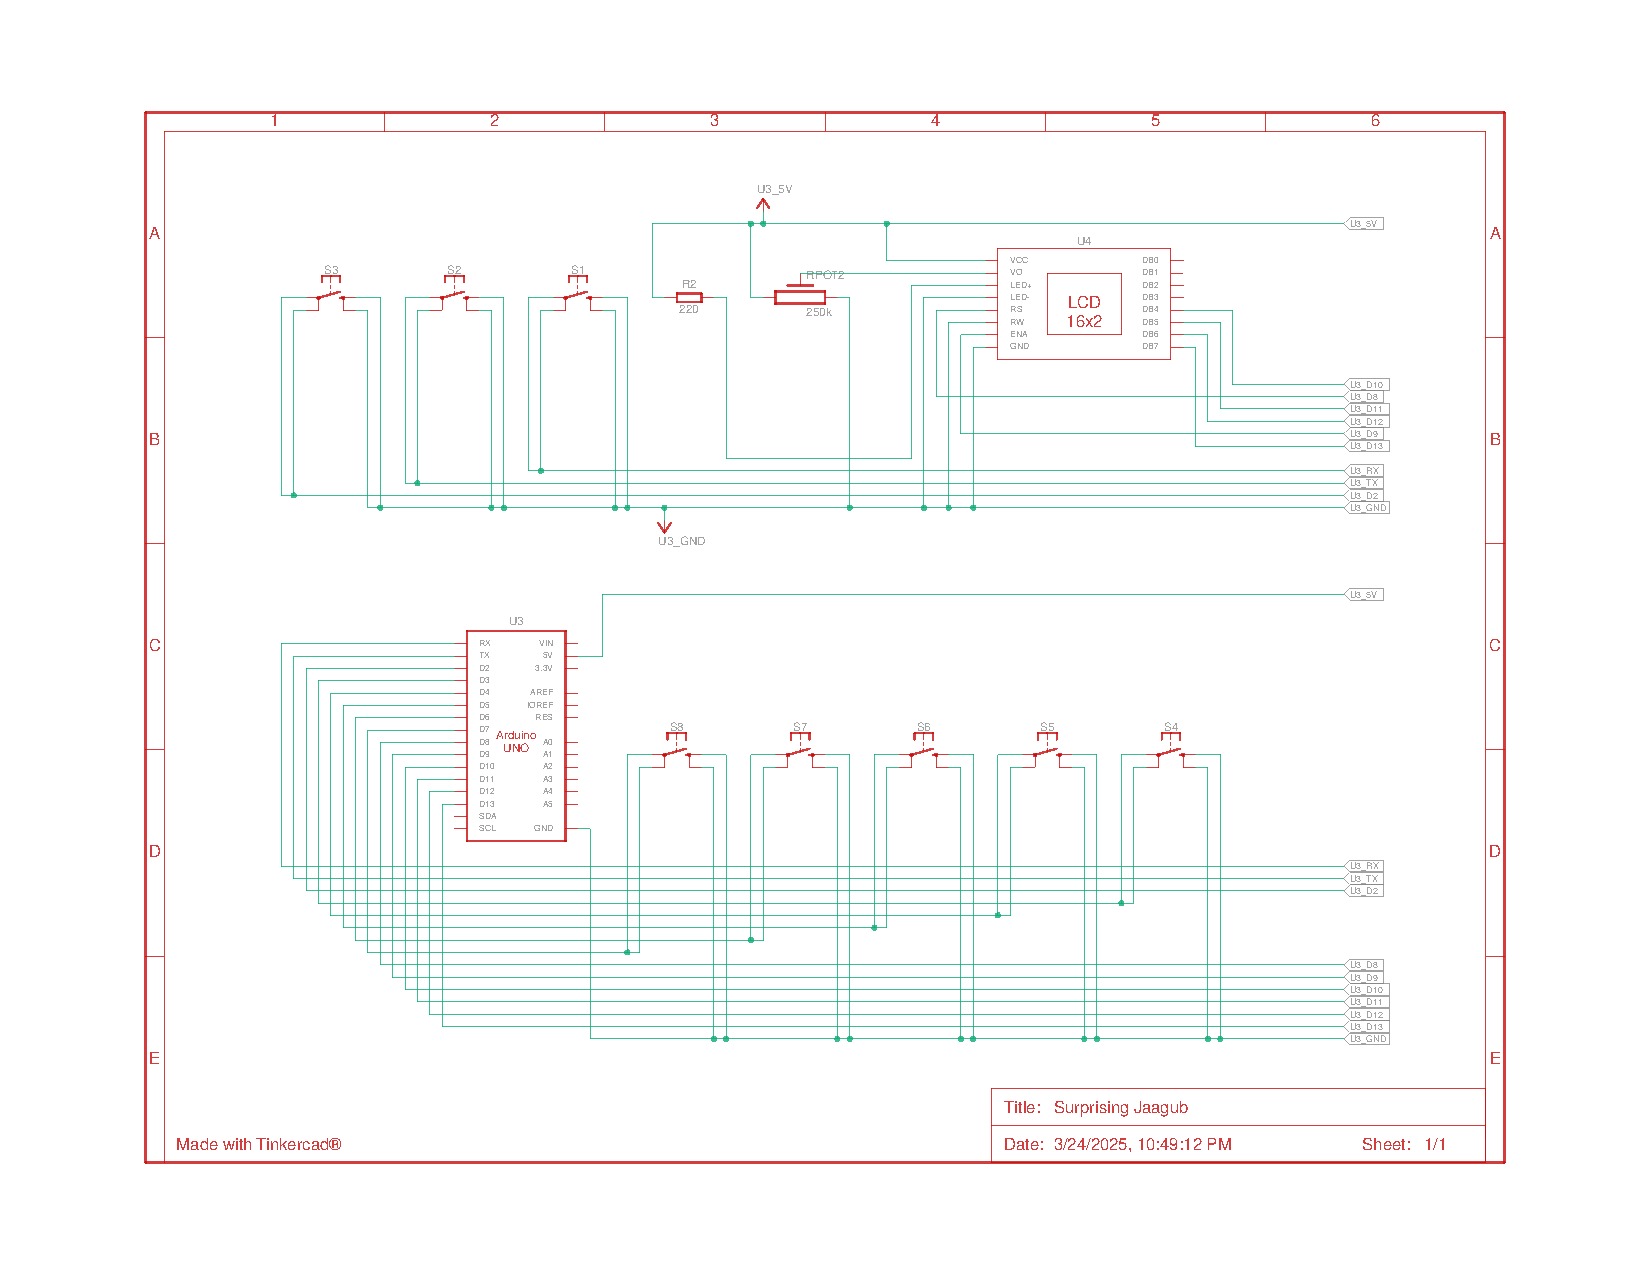
\includepdf{figs/calc.pdf}
	\begin{figure}[h!]
		\centering
		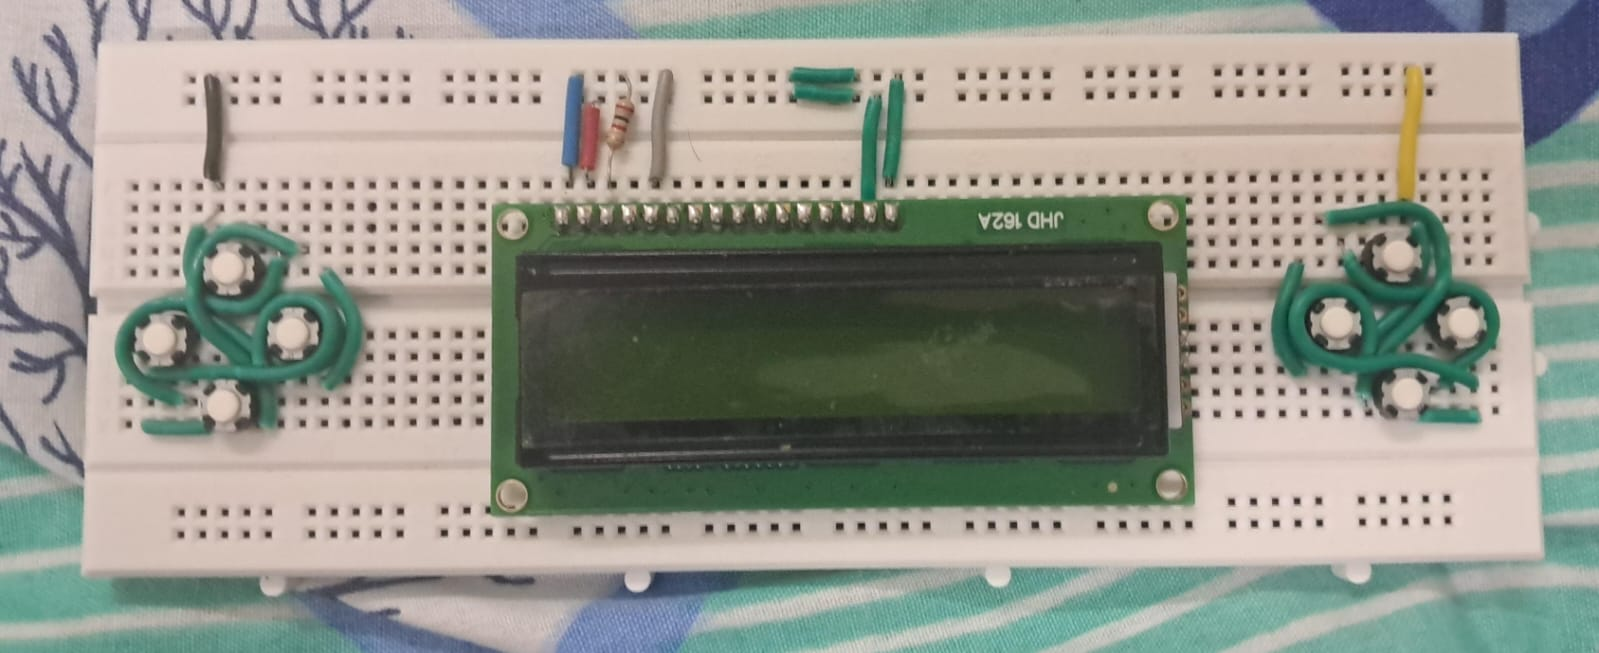
\includegraphics[width=0.8\textwidth]{figs/circuit.jpeg}
		\caption{Circuit Diagram}
	\end{figure}
	
	\section{User Modes}
	The calculator features four primary modes:
	\begin{enumerate}
		\item Number Mode: Allows input of numerical values from 0 to 9.
		\item Operators Mode: Includes basic arithmetic operators [+, -, *, /, e, pi, ), (, . , , ].
		\item Functions Mode: Offers common mathematical functions (sin, cos, tan, log, ln, pow,exp).
		\item Inverse Functions Mode: Provides inverse operations for functions (asin, acos, atan).
	\end{enumerate}
	
	\section{Control Logic}
	The first D-pad controls cursor movement (left and right buttons) and expression selection buttons are up and down. In the second D-Pad's left button acts as a delete key which removes the previous element from the cursor position, whereas the right button will solve for the expression. The second D-Pad's up and down buttons allow you to scroll through the modes.
	\section{User Interface}
	First, we have to set the mode. Then we use the first d-pad to cycle through the respective mode's list. Then we just pressed the forward cursor to move to the next expression. The cursor will accurately display where current expression. Now repeating the following process will give us the required expression to be calculated. Even though this may seem to be redundant and slow, with usage and over time, this process can be done really fast. While scrolling through the modes, we can see which mode is currently set at the corner of the screen in the second line.
		\begin{figure}[h!]
		\centering
		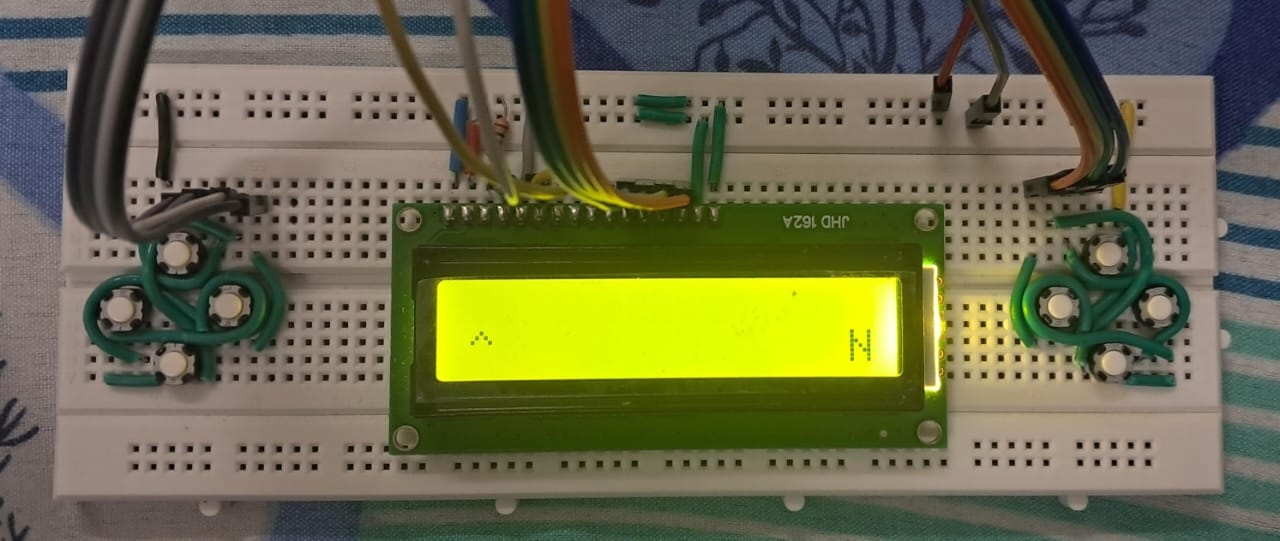
\includegraphics[width=0.8\textwidth]{figs/inter.jpeg}
		\caption{Interface Example 1, Showing the cursor and the mode indicator}
	\end{figure}
			\begin{figure}[h!]
		\centering
		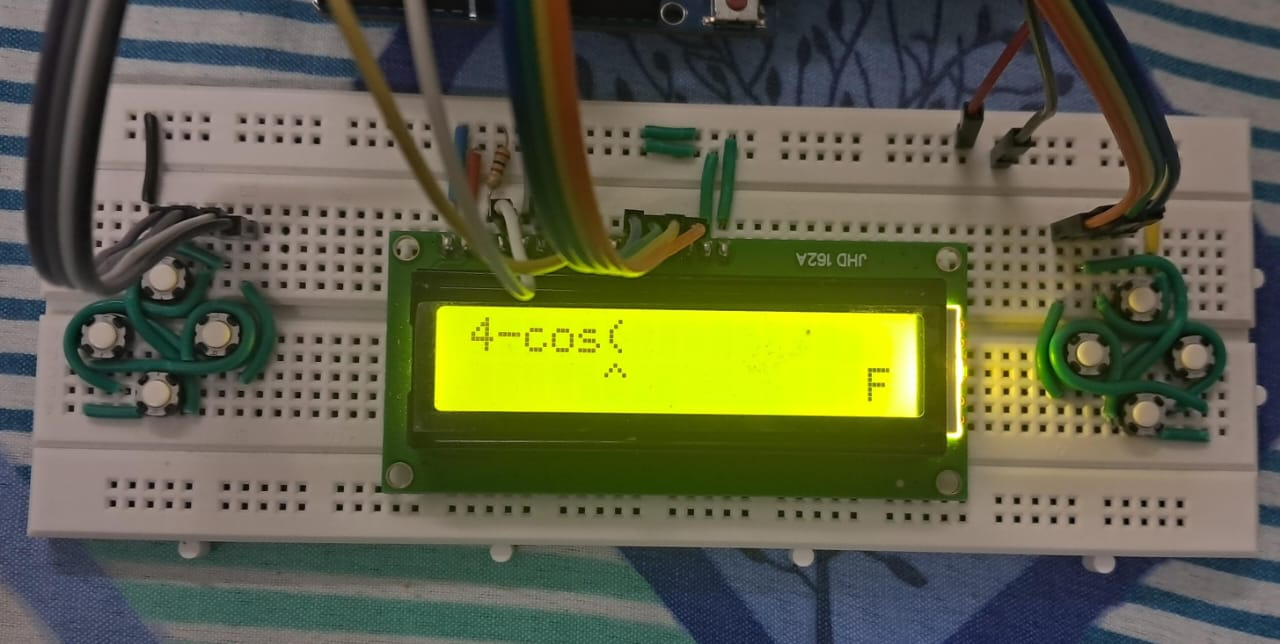
\includegraphics[width=0.8\textwidth]{figs/inter1.jpeg}
		\caption{Interface Example 2}
	\end{figure}
			\begin{figure}[h!]
		\centering
		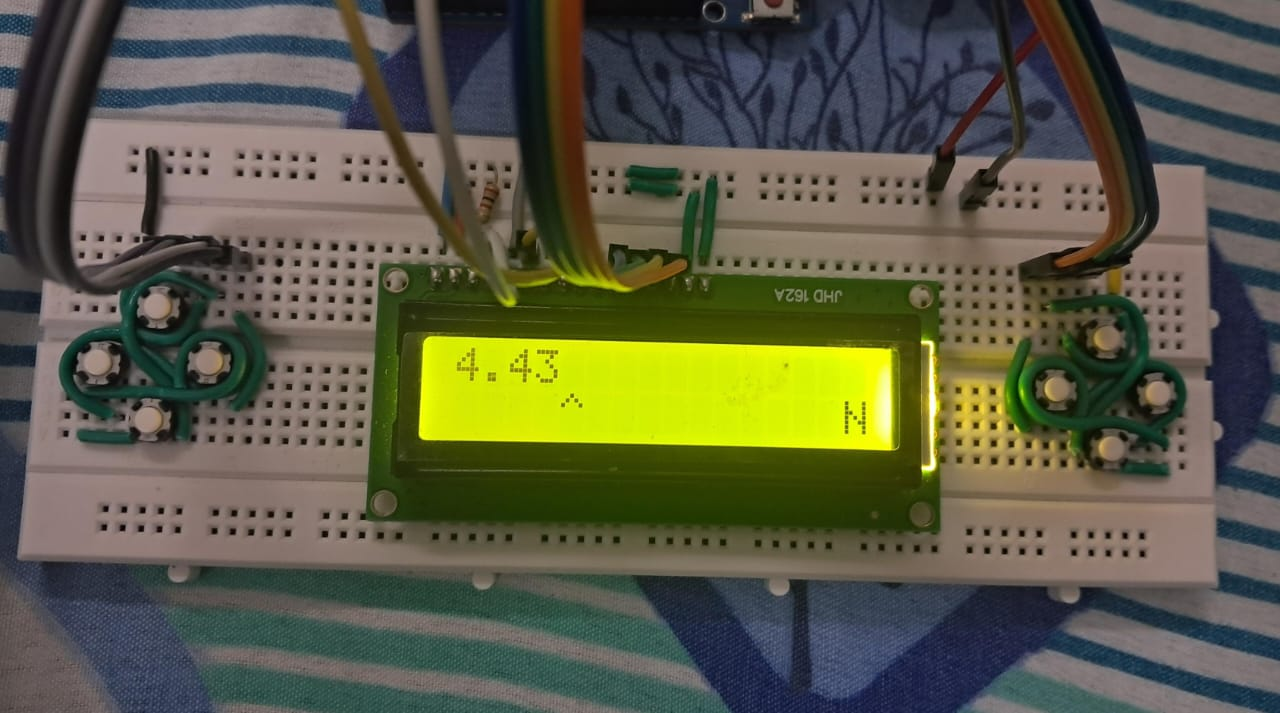
\includegraphics[width=0.8\textwidth]{figs/inter2.jpeg}
		\caption{Interface Example 3}
	\end{figure}
	\section{Expression Parser}
	I have used a library called tinyexpr.c , which allows you to parse the expression that we need to calculate. This tool allows you to calculate expressions with complex bodmas and nested function with ease and it comes with error handling. Ex. "$\sin(1/cos(\pi/3))/\log(pow(2, \pi/2))$". This library doesn't innately support being uploaded on the arduino due to it's large size despite being called "tinyexpr". After removing redundant libraries and codes used by tinyexpr and heavily modifying, it works without a problem on the Arduino. The .hex file is now just below 18kb which is the average .hex file size of the code made by majority of the class excluding the fact that, this parser is better than theirs and also features error handling.
	\section{Error Handling}
	If any expression has a mistake in it, Ex. incomplete operators, missing parenthesis etc, the calculator will pop up an error screen showing the pointing to the error in the expression, and then it goes back into input mode. 
	\begin{figure}[h!]
		\centering
		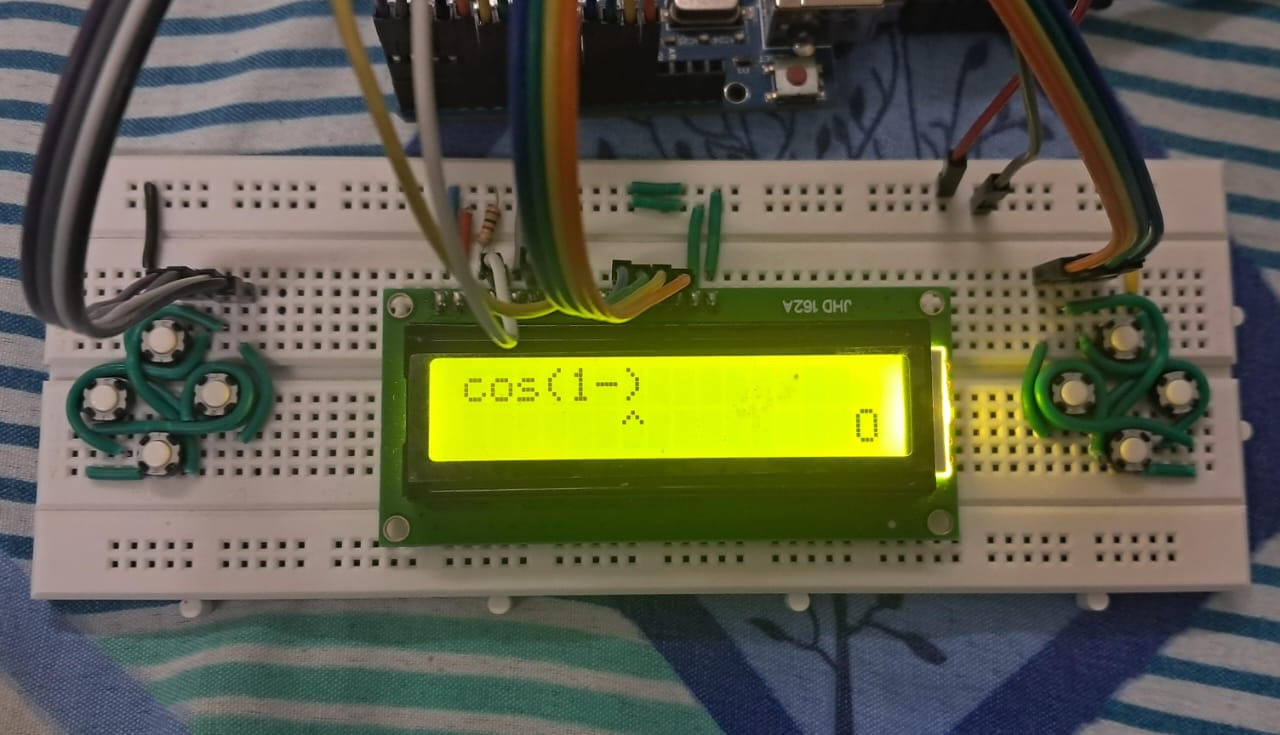
\includegraphics[width=0.8\textwidth]{figs/interp1.jpeg}
		\caption{Erred Prompt 1}
	\end{figure}
			\begin{figure}[h!]
		\centering
		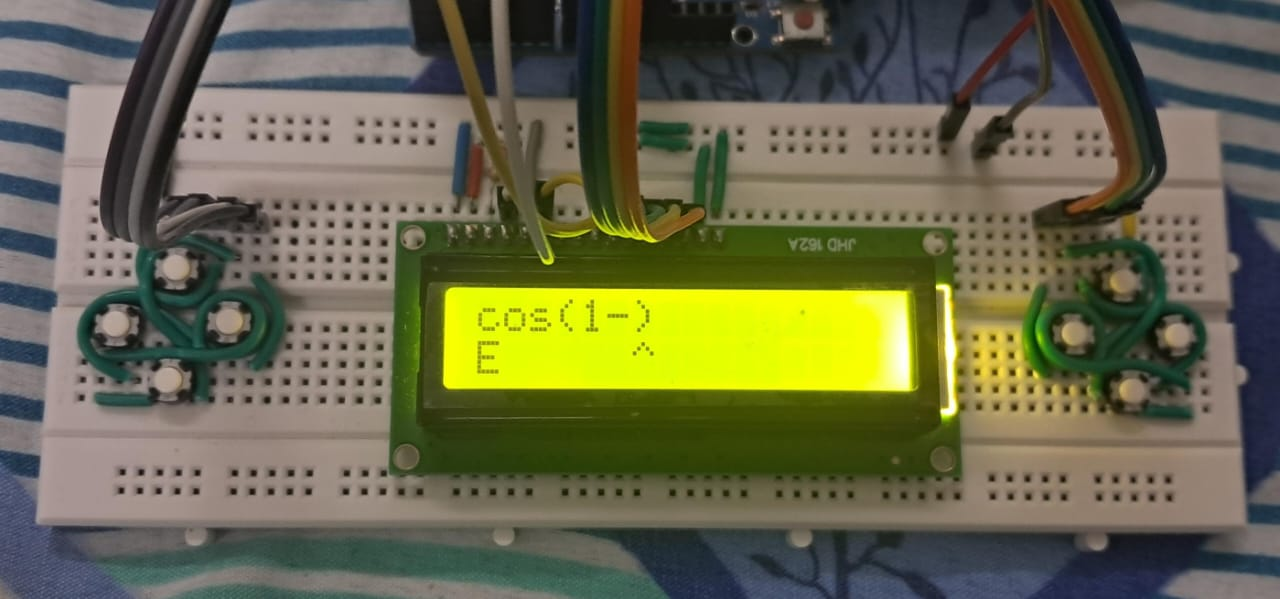
\includegraphics[width=0.8\textwidth]{figs/e1.jpeg}
		\caption{Error Indicator 1}
	\end{figure}
		\begin{figure}[h!]
		\centering
		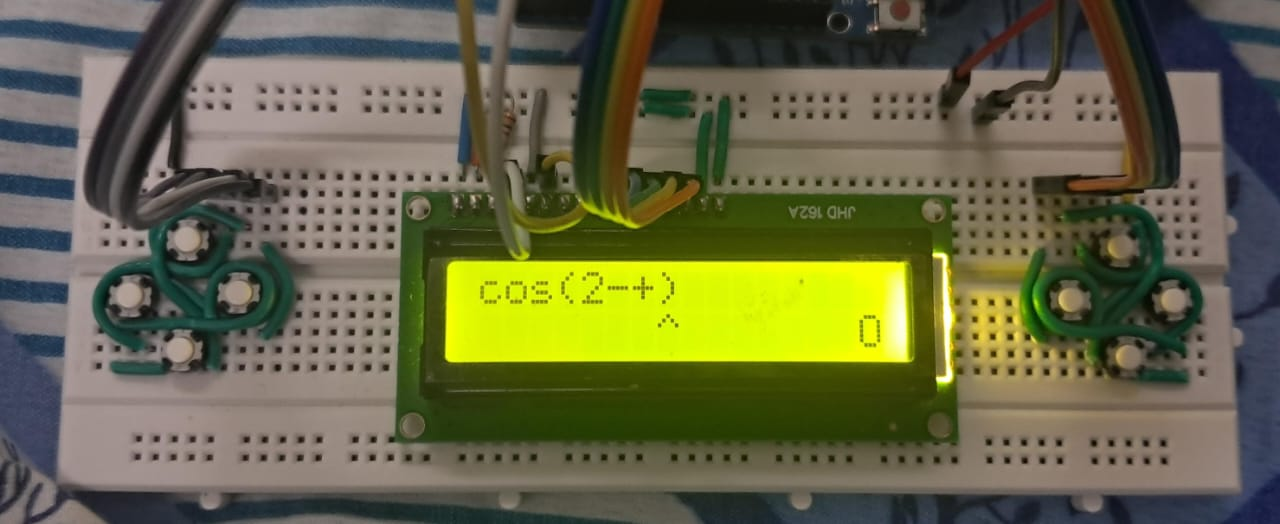
\includegraphics[width=0.8\textwidth]{figs/interp2.jpeg}
		\caption{Erred Prompt 2}
	\end{figure}
	\begin{figure}[h!]
		\centering
		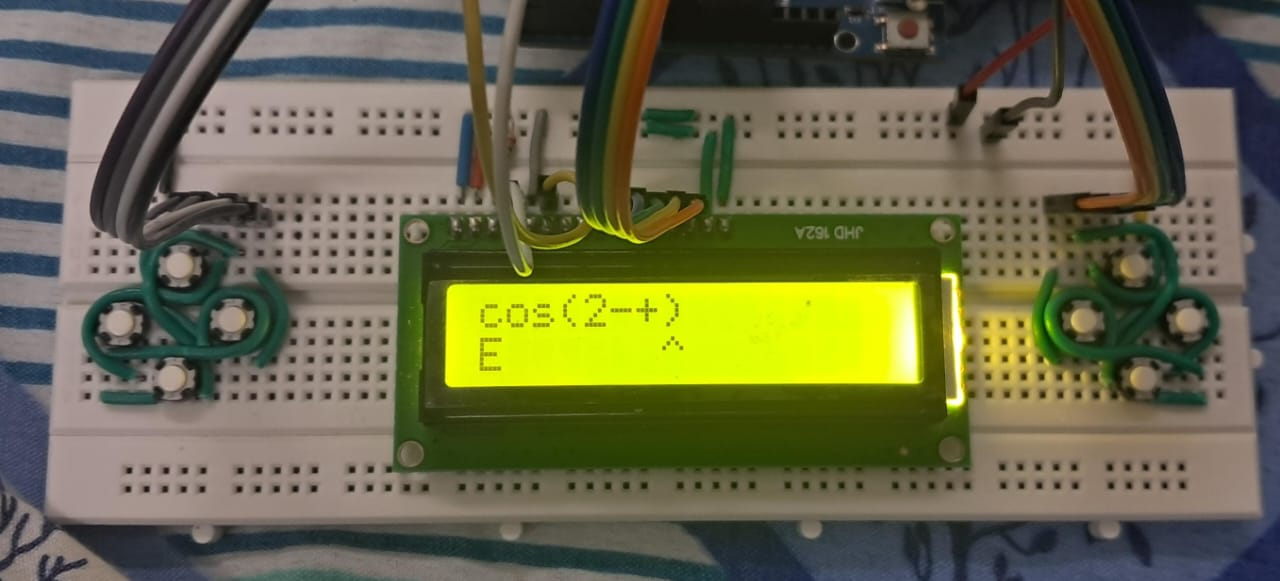
\includegraphics[width=0.8\textwidth]{figs/e2.jpeg}
		\caption{Error Indicator 2}
	\end{figure}
	\newpage
	\section{EEPROM Persistance}
	EEPROM persistence is implemented to store user data when the device is powered off. The expression, length of the expression and the cursor location is stored in the EEPROM.
	\section{Assembly Routines}
	To drive the LCD, I have implemented assembly routines. The following functions are present in the routines file.
	\begin{enumerate}
		\item SendNibble()
		\item SendByte()
		\item LCDCmd()
		\item LCDInit()
		\item LCDChar()
	\end{enumerate}
	The file is located at, \\
	\fbox{%
		\parbox{\textwidth}{
			/codes/final/routines.S
		}%
	} The makefile will automatically compile these routines with the embedded C code.
	
	\section{Function Implementations}
	I have implemented the following functions using the numerical methods.
\subsection{sin(x)}
I have used the Forward Euler method for estimating \(\sin(x)\). 
\begin{align}
	\frac{d^2 y_n}{d x_n^2} &= -y_n 
\end{align}

Using the finite difference approximation for the second derivative,

\begin{align}
	\frac{y_{n+1} - 2y_n + y_{n-1}}{h^2} &= -y_n
\end{align}

Rearranging for \( y_{n+1} \),

\begin{align}
	y_{n+1} &= 2y_n - y_{n-1} - h^2 y_n
\end{align}
The initial points are $y_0 = 0, y_1 = 0.099, h=  0.01$
\subsection{cos(x)}
 The same update equation for sin(x) is used, but this time $y_0 = 1, y_1 = 0.99, h= 0.01$.
\subsection{tan(x)}
I have used the second-order Runge-Kutta (RK2) method to approximate \(\tan(x)\). The differential equation governing \(\tan(x)\) is:

\begin{align}
	\frac{dy_n}{dx_n} = 1 + y_n^2
\end{align}

Using the RK2 method, the update steps are:

\begin{align}
	k_1 &= (1 + y_n^2) h, \\
	k_2 &= \left(1 + \left(y_n + \frac{k_1}{2} \right)^2 \right) h, \\
	y_{n+1} &= y_n + \frac{k_2 + k_1}{2}.
\end{align}
The above is the update equation for tan(x), where the initial conditions are, $y_0 =0, h = 0.01$.
\subsection{ln(x)}
I have used the second-order Runge-Kutta (RK2) method to approximate \(\ln(x)\). The governing differential equation is:

\begin{align}
	\frac{dy}{dx} = \frac{1}{x}
\end{align}

Applying the RK2 method:

\begin{align}
	k_1 &= \frac{1}{x_n}h,  \\
	k_2 &= \frac{1}{x_n + \frac{h}{2}} h, \\
	y_{n+1} &= y_n + \frac{k_2+k_1}{2}
\end{align}
The initial conditions are, $y_0 = -4.6, x_0 = 0.01, h = 0.01$
\subsection{log(x)}
Since \(\log(x) = \log(e)\ln(x)\), we use the same update equation as \(\ln(x)\) and then scale the function by $\log(e)$
\subsection{exp(x)}
The governing equation for \(e^x\) is:

\begin{align}
	\frac{dy}{dx} = y
\end{align}

Applying RK2:

\begin{align}
	k_1 &= y_n h, \\
	k_2 &= (y_n + \frac{k_1}{2})h, \\
	y_{n+1} &= y_n +\frac{k_1 + k_2}{2}.
\end{align}
Here the initial conditions are, $y_0 = 1, x_0 = 0, h = 0.01$

\subsection{pow(a, x)}
Since \( a^x = e^{x \ln a} \), we use the equation:

\begin{align}
	\frac{dy}{dx} = y \ln a
\end{align}

Applying RK2:

\begin{align}
	k_1 &= y_n \ln a h, \\
	k_2 &= (y_n + \frac{k_1}{2}) \ln a h, \\
	y_{n+1} &= y_n + \frac{k_1 + k_2}{2}.
\end{align}
Here the initial conditions are the same as the conditions for $exp(x)$
\subsection{asin(x)}
I have used Newton’s method to approximate \(\sin^{-1}(x)\). The governing equation is:

\begin{align}
	f(y) &= \sin(y) - x
\end{align}

Applying Newton’s iteration formula:

\begin{align}
	y_{n+1} &= y_n - \frac{\sin(y_n) - x}{\cos(y_n)}
\end{align}

This iterative formula refines the approximation of \(\sin^{-1}(x)\). The initial condition taken is $y_0  =x$.

\subsection{acos(x)}
Since \(\cos^{-1}(x)\) satisfies:

\begin{align}
	f(y) &= \cos(y) - x
\end{align}

The Newton’s update equation is:

\begin{align}
	y_{n+1} &= y_n - \frac{\cos(y_n) - x}{-\sin(y_n)}
\end{align}

which ensures convergence to \(\cos^{-1}(x)\). The initial condition taken is $y_0 =x$.

\subsection{atan(x)}
For \(\tan^{-1}(x)\), the equation is:

\begin{align}
	f(y) &= \tan(y) - x
\end{align}

Applying Newton’s method:

\begin{align}
	y_{n+1} &= y_n - \frac{\tan(y_n) - x}{\sec^2(y_n)}
\end{align}

This iterative approach provides an efficient method for computing \(\tan^{-1}(x)\). The initial condition taken is $y_0 =x$.


	\section{Conclusion}
	This calculator system effectively integrates a user-friendly interface with versatile mathematical capabilities, making it a practical tool for educational and everyday use.
	
	\section{Code Requirements}
	The code is located in the following directory:\\  
	\fbox{%
		\parbox{\textwidth}{
			/codes/final/code.c
		}%
	} It can be compiled and uploaded directly using the Makefile.
	
\end{document}
